\label{sec:evaluation}

This section answers the following questions:
\begin{itemize}
\item
  How effective is \Predator{} at detecting and predicting false sharing (Section~\ref{sec:effective})?

\item
  What is the performance (Sections~\ref{sec:perfoverhead}) and memory overhead of \Predator{} (\ref{sec:memoverhead})?

\item 
  How sensitive is \Predator{} on sampling rate (Section~\ref{sec:sensitivity})? 
 
\end{itemize}

\paragraph{Experimental Platform} All evaluations are performed on a quiescent Intel Core 2 dual-processor system equipped with 
16GB RAM. Each processor is a 4-core 64-bit Intel Xeon running at 2.33 GHz with a 4MB shared L2 cache and 32KB private L1 cache. The underlying operating system is unmodified CentOS 5.5, running with Linux kernel version 2.6.18-194.17.1.el5. The glibc version is 2.5. %since we can not report line number of source code with optimization level larger than ``-O2''.

\paragraph{Evaluated Applications} 
This paper evaluates two popular benchmark suites,
Phoenix (with large input) ~\cite{phoenix-hpca} and PARSEC (with simlarge input) ~\cite{parsec}. Even with unmodified LLVM-3.2, Facesim can not be compiled successfully (with complaints on an undefined template) and Canneal aborts unexpectedly. Thus, these two benchmarks are excluded here.
We also evaluate \Predator{} on six real applications, including \texttt{MySQL, Boost, Memcached, aget, pbzip2} and \texttt{pfscan}.

In order to compare performance fairly, all benchmarks were built as 64-bit executables 
using LLVM compiler (clang-3.2) with optimization level ``-O1''.

\subsection{Detection and Prediction Effectiveness}
\label{sec:effective}

\Predator{} precisely report false sharing problems. Figure~\ref{fig:lrreport} shows an example, generated by \Predator{} for the \texttt{linear\_regression} benchmark. From this report, we can see clearly that the heap object starting with $0x40000038$ causes a large number of cache invalidations potentially. The stack of allocation callsite is provided to help locate culprits. In addition, \Predator{} also reports word level access information of this object, which helps to identify where false sharing occurs. For this example, since different threads are accessing different cache lines, which is a latent false sharing problem predicted by \Predator{}. 

\begin{figure*}[!ht]
{\centering
\subfigure{\lstinputlisting[numbers=none,frame=none,boxpos=t]{fig/linearregression.report}}
\caption{False sharing report for the \texttt{linear\_regression} benchmark.
\label{fig:lrreport}}
}
\end{figure*}

\subsubsection{Benchmarks}
\label{sec:benchmarks}
Detection results on two benchmark suites, Phoenix and PARSEC, are listed in the Table~\ref{table:detection}. 

\begin{table*}[ht!]
{\centering\begin{tabular}{l|r|r|r|r|r}\hline
{\bf \small Benchmark} & {\bf \small Source Code} & {\bf \small New} & {\bf \small Without Prediction} &{\bf \small With Prediction} & {\bf \small Improvement} \\
\hline
\small \textbf{histogram} & {\small histogram-pthread.c:213} & \cmark{} &\cmark{} & \cmark{} & 46.22\%\\
\small \textbf{linear\_regression} & {\small linear\_regression-pthread.c:133} & & & \cmark{} & 1206.93\% \\
\small \textbf{reverse\_index} & {\small reverseindex-pthread.c:511} & & \cmark{} & \cmark{} & 0.09\%\\
\small \textbf{word\_count} & {\small word\_count-pthread.c:136} & & \cmark{} & \cmark{} & 0.14\%\\
\hline
\small \textbf{streamcluster} & {\small streamcluster.cpp:985} &  & \cmark{} & \cmark{} &7.52\% \\
\small \textbf{streamcluster} & {\small streamcluster.cpp:1907} & \cmark{} & \cmark{} & \cmark{} & 4.77\%\\
\hline
\end{tabular}
\caption{False sharing problems of Phoenix and PARSEC benchmark suites. \label{table:detection}}
}
\end{table*}

In this table, the first column lists those programs with false sharing problems.  The second column shows precisely where the problem is. Since all discovered false sharing occurs inside the same heap object, we list callsite source code information in this column.  The third column ``New'' marks whether this false sharing was newly
discovered by \Predator{} or not.  A checkmark in the appropriate
column indicates whether the false sharing was identified without
prediction and/or with prediction.  The final column, ``Improvement'',
shows the performance improvement after fixing false sharing.
%The number is based on the average runtime of $10$ runs. 

As shown in the table, \Predator{} reveals two unknown false sharing problems. 
It is the first tool to detect the false sharing problem in \texttt{histogram} 
and in line $1908$ of \texttt{streamcluster}. 
In \texttt{histogram}, multiple threads repeatedly modify different locations of the same heap object. 
Padding the data structure \texttt{thread\_arg\_t} fixes the false sharing problem and improves the performance around 46\%. In \texttt{streamcluster}, multiple threads are simultaneously accessing and updating the same \texttt{bool} array, \texttt{switch\_membership}. By simply changing this array to \texttt{long} type contributes to about 4.7\% performance improvement.

%, although it is not a complete fix of false sharing. 
%None of these two false sharing problems has been reported by previous tools.
All other false sharing problems have been discovered by previous tools~\cite{sheriff}. We do not see much performance improvement for \texttt{reverse\_index} and \texttt{word\_count} benchmarks, but they are reported because the number of cache invalidations 
reaches our predefined threshold.
Making reporting threshold higher can avoid the report of insignificant false sharing problems.
It is worth noting that these two benchmarks definitely have false sharing problems,
which has been confirmed by \Sheriff~\cite{sheriff} and can be confirmed by word level information outputted by \Predator{} too. 

\texttt{streamcluster} has another false sharing problem at line $985$. Different threads change the same object (\texttt{work\_mem}) simultaneously. Authors of \texttt{streamclsuter} have already realized possible false sharing problems and meant to utilize a macro \texttt{CACHE\_LINE} to avoid it. Unfortunately, the defaulted value of this macro is set to $32$ bytes, which is different with the actual cache line size of our hardware. By setting to $64$ bytes instead, we achieve around $7.5\%$ performance improvement.

\texttt{linear\_regression} has a severe false sharing problem, while fixing it improves the performance more than $12\times$. In this benchmark, different threads update their thread specific locations inside a heap object(\texttt{tid\_args}) in a tight loop,  causing a huge amount of cache invalidations. For this benchmark, Nanavati et al.~\cite{OSdetection} observe that false sharing occurs when using \texttt{clang} and disappears when using gcc with optimization levels -O2 and -O3. However, we observe a different result on \texttt{clang} when using our customized memory allocator. As shown in Figure~\ref{fig:lrreport}, there is no observed false sharing problem when using \texttt{clang-3.2} at ``-O1'' optimization level. This phenomenon actually exemplifies the necessity of a predictive detection tool. 

\subsubsection{Real Applications}
To verify \Predator{}'s practicality, we further evaluate it on several widely-used real applications, whereas none of previous work has done this. These real applications include a server application (MySQL~\cite{mysql}),
a standard C++ library (Boost~\cite{libfalsesharing}),
a distributed memory object caching system (\texttt{memcached}), a network retriever (\texttt{aget}),
a parallel bzip2 file compressor (\texttt{pbzip2}), and a parallel file scanner (\texttt{pfscan}).

For MySQL and Boost, we evaluate on two specific versions, MySQL-5.5.32 and boost-1.49.0, which are known to have some false sharing problems. Other applications includes \texttt{memcached-1.4.15, aget-0.4.1} and \texttt{pbzip2-1.1.6}.

The false sharing problem of MySQL has caused a significant scalability problem and was very difficult to identify.
According to the architect of MySQL Mikael Ronstrom, ``we had gathered specialists on InnoDB..., participants from MySQL support... and a number of generic specialists on 
computer performance...'', ``the fruit of the meeting ... were able to improve MySQL performance by 6$\times$ with those scalability fixes''~\cite{mysql}. 
The false sharing of \texttt{Boost} library is caused by the usage of \texttt{spinlock} pool. Different threads may utilize different spinlocks located in the same cache line in this case. Fixing it brings a 40\% performance improvement.
\Predator{} is able to successfully detect false sharing locations in both \texttt{MySQL} and the \texttt{Boost} library. 
For the other four applications, \Predator{} does not find severe false sharing problems.

\subsubsection{Prediction Effectiveness}
\label{sec:predicteval}
Predictive detection reveals un-observed false sharing problems. In this section, we further verify whether prediction can always identify false sharing problems without occurrences.

\texttt{linear\_regression} benchmark is selected here because of the following two reasons:
\begin{enumerate}
\item
The false sharing problem of this benchmark cannot be detected without prediction; 
\item
False sharing severely degrades performance when it actually occurs. Hence, it is a serious problem that should always be detected. 
\end{enumerate}

\begin{figure}[!ht]
{\centering
\subfigure{\lstinputlisting[numbers=none,frame=none,boxpos=t]{fig/linearregression.psedocode}}
\caption{False sharing problem inside \texttt{linear\_regression} benchmark.
\label{fig:linearregression}}
}
\end{figure}

Figure~\ref{fig:linearregression} shows the data structure and source code exercising appropriate false sharing. The size of this data structure, \texttt{lreg\_args}, is $64$ bytes 
when we use \texttt{clang} to compile a $64$-bit binary at the ``-O1'' optimization level. For this benchmark, the main thread allocates an array with the number of elements equalling to the number of underlying hardware cores. Each element is a \texttt{lreg\_args} type with $64$ bytes. Then this array is passed to different threads (\texttt{lreg\_thread}) so that each thread only updates its thread-dependent area. False sharing occurs if two threads happens to update data in the same cache line. 

Figure~\ref{fig:perfsensitive} shows how sensitive  of the performance is to different starting address of false sharing object. When the offset is $0$ or $56$ bytes, this benchmark achieves its optimal performance and has no false sharing at all. When the offset is $24$ bytes, this benchmarks runs around $15$ times slower than its optimal performance because of false sharing problem.

Our evaluations show that \Predator{} can always detect the false sharing problem inside with prediction enabled, demonstrating its effectiveness.

\subsection{Performance Overhead}
\label{sec:perfoverhead}

\begin{figure*}[ht]
\begin{center}
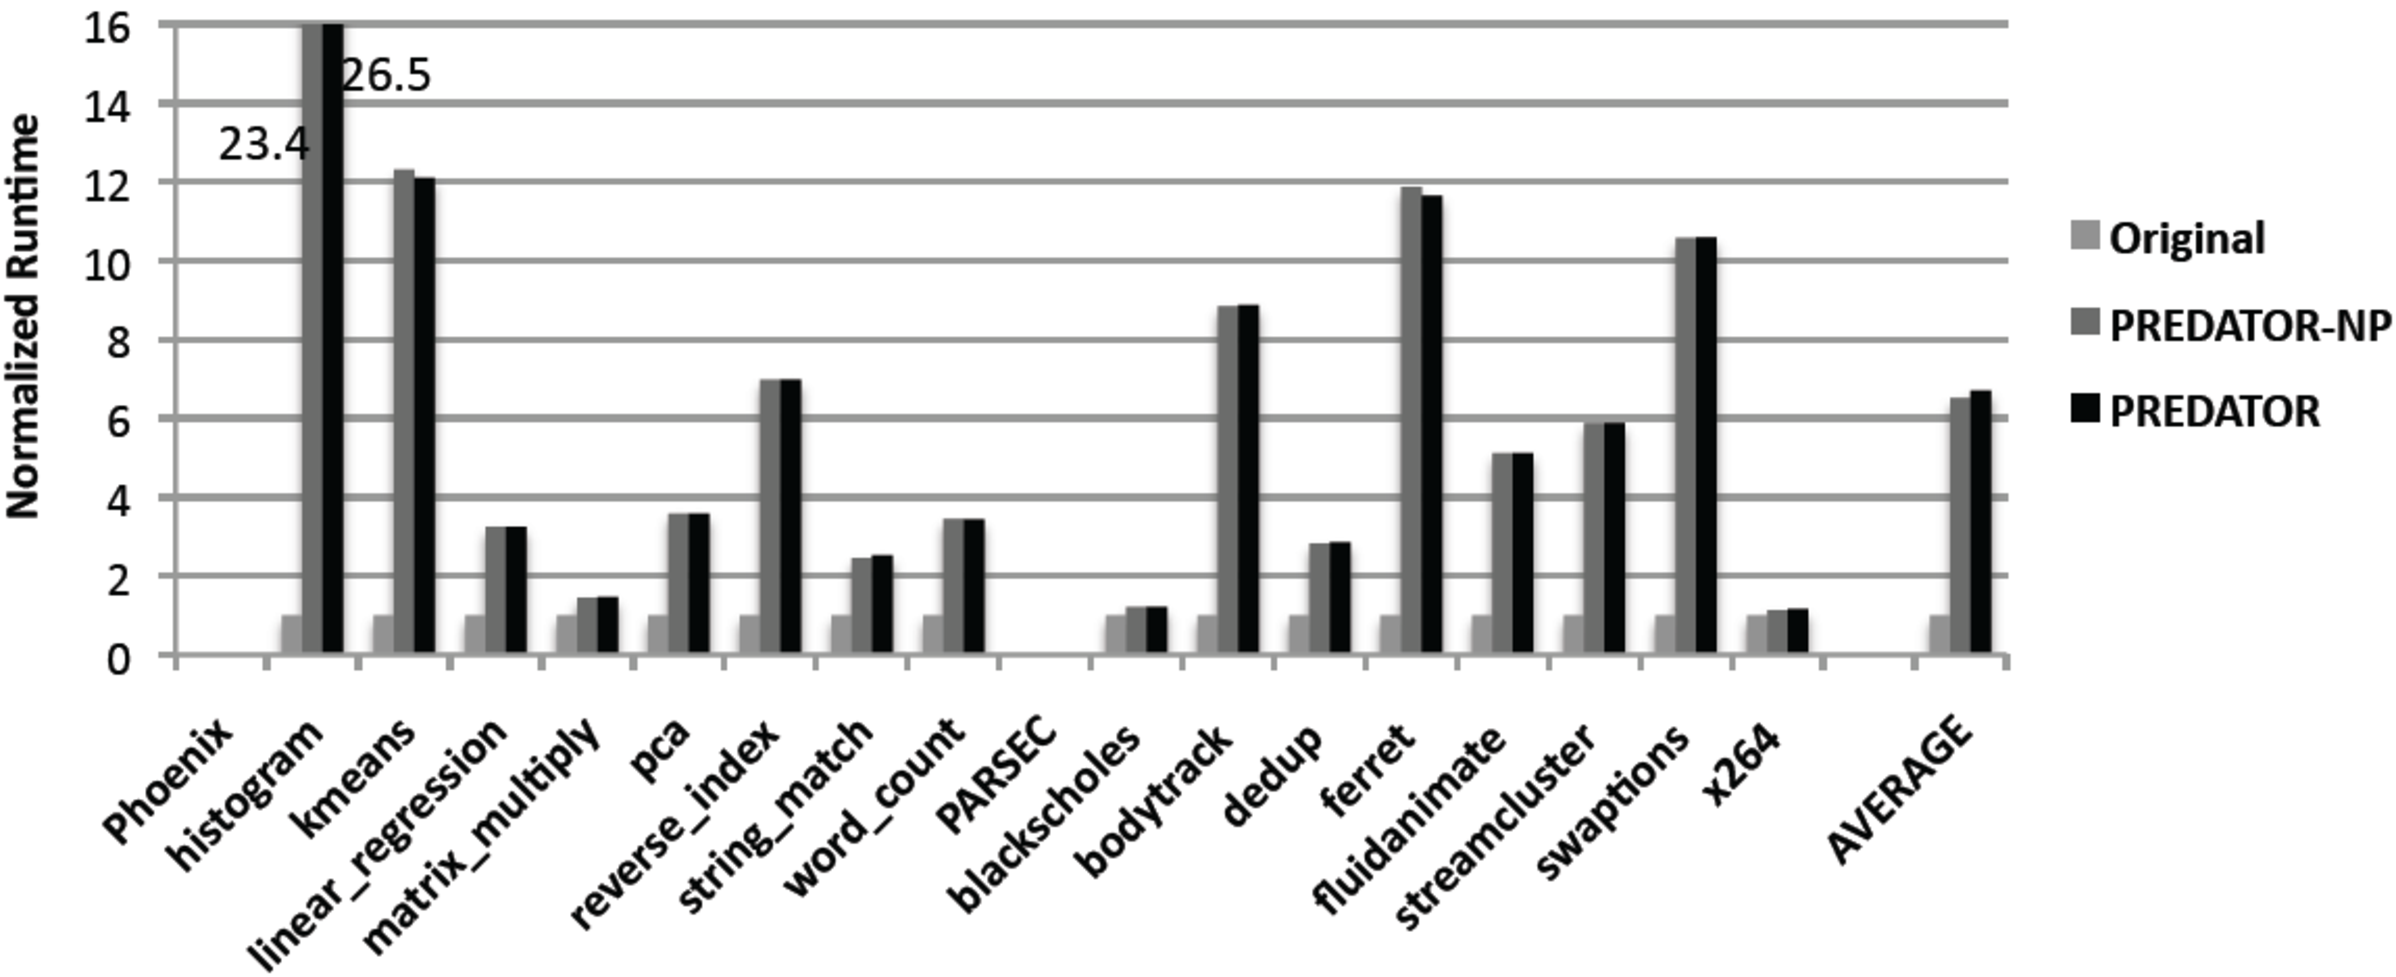
\includegraphics[width=6.5in]{fig/perf}
\end{center}
\caption{
Performance overhead of \Predator{} with and without prediction(PREDATOR-NP).
\label{fig:perf}}
\end{figure*}

To avoid the effect caused by extreme outliers, all performance data shown in this section
is based on the average of $10$ runs while excluding the maximum and minimum values. Actual performance is shown in Figure~\ref{fig:perf}. 

For $16$ benchmarks from Phoenix and PARSEC benchmark suites and six real applications,  \Predator{} imposes around $5.4\times$ performance overhead. There is no big difference on performance when disabling the prediction mechanism. 
 
Among these programs, five of them have more than $8\times$ performance overhead, including \texttt{histogram, kmeans, bodytrack, ferret} and \texttt{swaptions}. 
Program \texttt{histogram} runs more than $26$ slower than original executions with \pthreads{} library, which is caused by a severe false sharing problem inside. Tracking detailed access for cache lines with false sharing exacerbates the false sharing effect (see more discussion of this in Section~\ref{sec:sample}).  For \texttt{bodytrack} and \texttt{ferret}, \Predator{} found a large amount of cache lines with writes larger than {\it Tracking-Threshold}, but there is no actual false sharing problem inside. Thus Tracking all accesses details for those cache lines imposes significant performance overhead. Currently, we cannot identify the reasons why \texttt{kmeans} runs much slower in \Predator{}.
   
We also observe that \Predator{} impose very minimum performance overhead for IO-bound applications, such as \texttt{matrix\_multiply}, \texttt{blackscholes}, \texttt{x264}, \texttt{aget}, \texttt{Memcached}, \texttt{pbzip2}, and \texttt{pfscan}.  

\subsection{Memory Overhead}
\label{sec:memoverhead}
We evaluate the physical memory overhead here because \Predator{} pre-allocates a 4 gigabytes block of heap initially. Proportional set size (PSS) in \texttt{/proc/self/smaps} reflects physical memory increase on the existing system by running an application~\cite{memusage}. Thus, we periodically collect this data and use the sum of different memory mappings as total physical memory usage. We presents the maximum value of physical memory usage in Figure~\ref{fig:memusage}. 

\Predator{} imposes less than 50\% memory overhead for 17 applications out of 22 applications.  For \texttt{swaptions} and \texttt{aget}, \Predator{} introduces significant memory overhead because original memory usage of these two benchmarks are too small, only $3$ kilobytes. Adding the code of detection, prediction and reporting contributes to a large portion of memory overhead. We are not clear why \texttt{MySQL} consume much more memory. Although the average memory usage of all applications is over $2\times$, the total memory usage overhead is only about $40\%$. 

\begin{figure*}
\begin{center} 
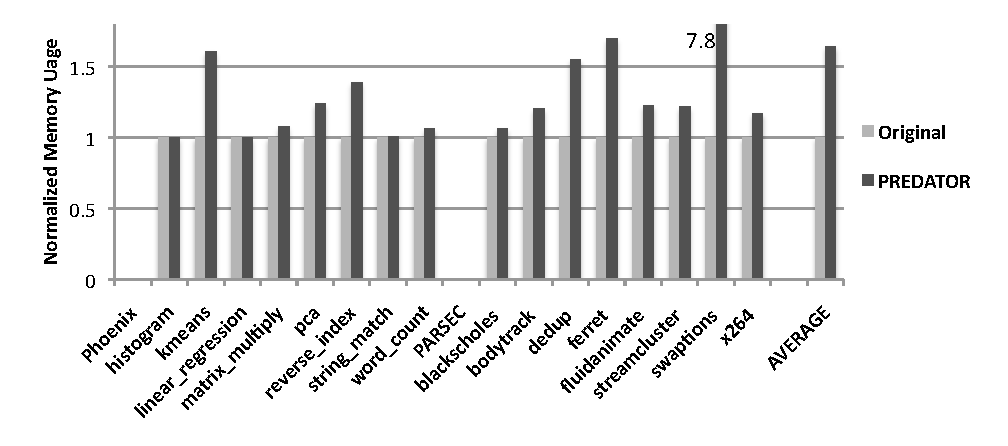
\includegraphics[width=6.5in]{fig/memusage}
\end{center}
%\includegraphics{fig/potential.pdf}
\caption{Memory usage overhead.}
\label{fig:memusage}
\end{figure*}


\subsection{Sensitivity on Sampling Rate}
\label{sec:sensitivity}
In Section~\ref{sec:sample}, we discuss that \Predator{} utilizes the sampling mechanism to reduce the performance overhead of detailed tracking. Different sampling rate do not effect the memory usage. Thus, we only evaluate the effect of sampling rate on performance and effectiveness. 

The default sampling rate of \Predator{} is 1\%. In this section, we also evaluate two other sampling rates, 0.1\% and 10\%. The performance results under three different sample rates are shown in Figure~\ref{fig:sample}. \Predator{} introduces less performance overhead under a lower sampling rate, which meets our expectation. For effectiveness, even using the 0.1\% sampling rate, \Predator{} can still detect all false sharing problems, but with a lower number of cache invalidations. 
 
\begin{figure}
\begin{center} 
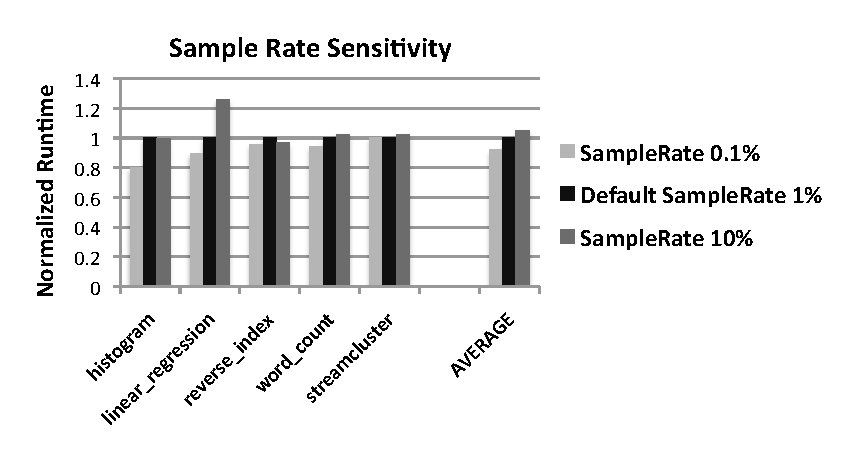
\includegraphics[width=3.4in]{fig/sample}
\end{center}
%\includegraphics{fig/potential.pdf}
\caption{Normalized Runtime for different sampling rates.}
\label{fig:sample}
\end{figure}


